\documentclass[12pt]{article}
\usepackage[spanish]{babel}

%%%%%%%%%%%%%%%%%%%%%%%%%%%%%%%%%%
%%%%%%%%%%%%%%%%%%%%%%%%%%%%%   %%
%%        Datos Trabajo     %%  %%
%%%%%%%%%%%%%%%%%%%%%%%%%%%%%%%%%%
\newcommand{\titulo}[0]{Evidencia de Aprendizaje}
\newcommand{\materia}[0]{Estadística Básica}
\newcommand{\grupo}[0]{BI-BEBA-2002-B2-013}
\newcommand{\unidad}[0]{Unidad 1}


%%%%%%%%%%%%%%%%%%%%%%%%%%%%%%%%%%
%%%%%%%%%%%%%%%%%%%%%%%%%%%%%%%%%%
\usepackage{amssymb}
\usepackage{booktabs}
\usepackage{enumerate}
\usepackage{geometry}
\usepackage{mathtools}
\usepackage{multicol}
\usepackage{soul}

\usepackage{graphicx}
	\graphicspath{ {assets/} }

\usepackage{hyperref}
	\hypersetup{
			pdftex,
		        pdfauthor={bench},
		        pdftitle={\titulo},
		        pdfsubject={\materia},
		        pdfkeywords={\grupo, \unidad, UnADM},
		        pdfproducer={Latex with hyperref, Ubuntu},
		        pdfcreator={pdflatex, or other tool},
			colorlinks=true,
				linkcolor=red,
				urlcolor=cyan,
				filecolor=green,
				citecolor=blue}

%%%%%%%%%%%%%%%%%%%%%%%%%%%%%%%%%%
%%%%%%%%%%%%%%%%%%%%%%%%%%%%%%%%%%

\title{
	
\includegraphics{../../../assets/logo-unadm} \\
	\ \\ Benjam\'in Rivera \\
	\bf{\titulo}\\\ \\}

\author{
	Universidad Abierta y a Distancia de México \\
	TSU en Biotecnolog\'ia \\
	\textit{Materia:} \materia \\
	\textit{Grupo:} \grupo \\
	\textit{Unidad:} \unidad \\
	\\
	\textit{Matricula:} ES202105994 }

\date{\textit{Fecha de entrega:} \today}


%%%%%%%%%%%%%%%%%%%%%%%%%%%%%
%%        Documento         %%
%%%%%%%%%%%%%%%%%%%%%%%%%%%%%%%
\begin{document}
\maketitle\newpage


\part*{Fase 1}


\section{Caso de estudio}


	\par Estoy interesado en estudiar las \textbf{t\'ecnicas de repoblaci\'on de ecosistemas} usando agentes biol\'ogicos. Uno de los t\'emas de interes para poder desarrollar esta investigaci\'on es conocer las \textbf{especies por espacio geogr\'afico} que habitan. Esto es importante para poder analizar ecosistemas afectados y aquellos que sean sanos, y que posean caracteristicas similares. 

	\begin{figure}[h]
		\centering
			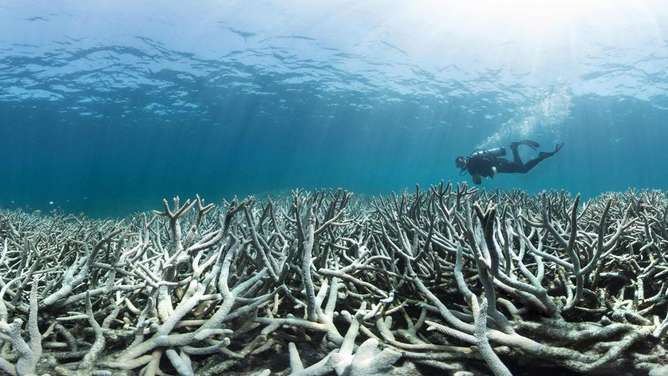
\includegraphics[width=0.6\textwidth]{coral-muerto.jpg}
		\caption{Corales muertos en el Océano Índico por culpa del calentamiento global \cite{corales muertos}}
		\label{fig: corales muertos}
	\end{figure}
	

	\par Entonces en \textbf{esta parte} nos centraremos en las \textbf{ubicaciones de los bancos de algas del mundo}. Esta informaci\'on nos pertmitira teorizar t\'ecnicas de \textit{biorremediaci\'on} en funci\'on de otros ambientes similares. Adem\'as, el estudio de estos en alg\'un tiempo determinado nos dara una oportunidad para identificar causas de infeccion y muerte de las agrupaciones de estos; para tratar de predecir los corales que esten en peligro por causas similares.

	\begin{figure}[p]
		\centering
			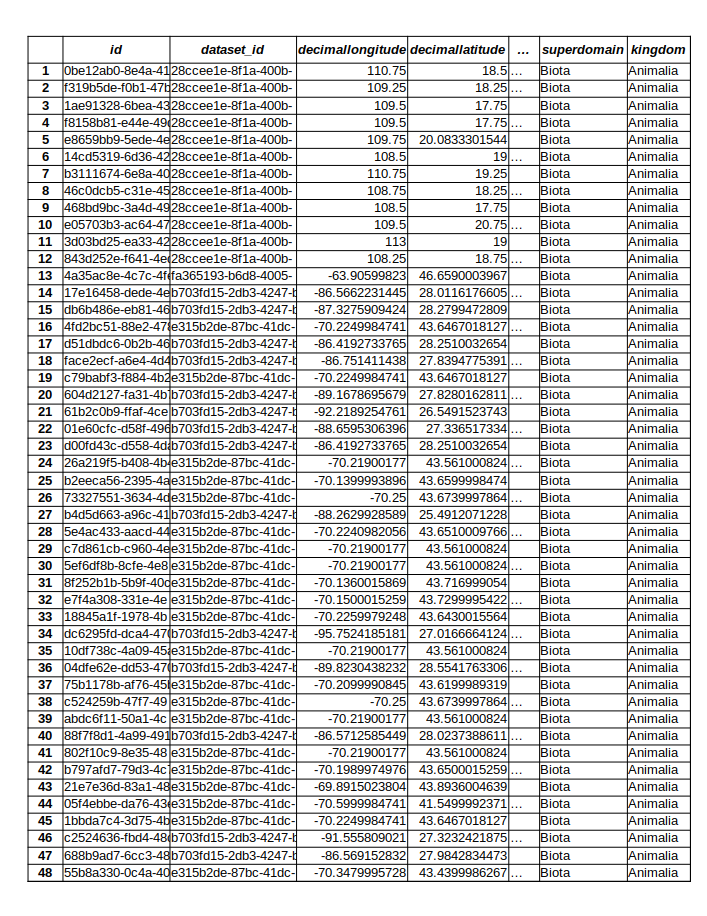
\includegraphics[width=0.98\textwidth]{tabla.png}
		\caption{Parte de los datos obtenidos de \cite{db}}
		\label{fig: tabla de datos}
	\end{figure}



\section{Base de Datos}
	
	\par Para poder estudiar la distribución de coral, y sus especies, en el mundo; usaremos la base de datos \cite{db}. Parte de los datos que contiene esta se pueden apreciar en la Figura~\ref{fig: tabla de datos}, esta \'unicamente contien parte de todo los datos que se pueden encontrar en la \textit{base de datos}. Luego con la informaci\'on obtenida se genero el mapa de la Figura~\ref{fig: coral en america}, la cual muestra la densidad de corales, en un momento determiando, en Am\'erica. 

	\subsection{Sobre la Base de Datos}
	
		\par La base de datos (\cite{db}) con la que vamos a trabajar tiene $221$ columnas, lo que se traduce en $221$ características, acerca de poblaciones de algas en todo el mundo. Las características contenidas incluyen las coordenadas geográficas (latitud y longitud), identificadores, fechas reales y estimaciones, información de la especie que habita, entre otras. En esta base de datos se tienen $65,080,440$ entradas, por lo que hay que tener cuidado para trabajar con esta; aunque por otro lado nos dará información más que suficiente para trabajar.
		
        \par Algunos de los datos cuantitativos que podemos identificar en esta base de datos son id, id del conjunto de datos, longitud, latitud, fecha de inicio, medida y término, además del año de registro, profundidad máxima y mínima de la agrupación, entre otros. A continuacu\'on se especificar\'a el nombre en donde se guardan algunas caracter\'isticas y se explicara brevemente lo que contienen:
        \begin{quote}\begin{description}
			\item [id] Este es un dato discreto, porque \'unicamente guardara enteros, para identifcar cada una de las entradas del archivo.
			\item [dataset id] Este tambi\'en es un dato descreto, porque \'unicamente guardara enteros, para identificar la fuente que ingreso el archivo.
			\item [decimallongitude] Este campo guarda la longitud de la cordenada de la muestra que se identific\'o, este es un dato continuo (dado que la posici\'on siempre puede ser m\'as precisa) 
			\item [decimallatitude] Aqui se guarda la latitud de la muestra. Dato continuo.
			\item [date\_start] Esta entrada guarda la fecha estimada 
			\item [minimumdepthinmeters] Profundidad minima de la agrupaci\'on de coral. Dato continuo.
			\item [maximumdepthinmeters] Profundidad maxima de la agrupaci\'on de coral. Dato continuo.
		\end{description}\end{quote}
		
		\par Para \textbf{este caso de estudio}\footnote{La ubicaciones de los bancos de algas del mundo} \'unicamente nos interesan las posiciones de los corales encontrados en la base de datos, esta informaci\'on se encuentra en la \textit{base de datos} bajo las columnas \textit{decimallatitude} y \textit{decimallongitud}. Y, como se mencion anteriormente, con estas generamos el gr\'afico de la Figura~\ref{fig: coral en america}.

		\begin{figure}[p]
			\centering
				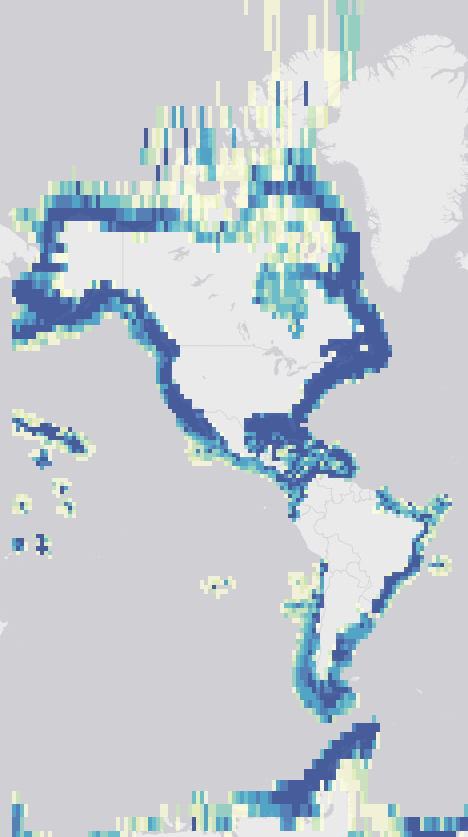
\includegraphics[width=0.7\textwidth]{coral-mundo.png}
			\caption{Representaci\'on de distribuci\'on de coral en Am\'erica. Datos obtenidos de \cite{db}}
			\label{fig: coral en america}
		\end{figure}


\section{Conclusi\'on}

	\par La recolecci\'on y el an\'alisis de datos parece ser una de las tareas m\'as complejas e importantes de cualquier proyecto de investigaci\'on. Adem\'as de que con la creciente velocidad actual de creaci\'on de esta actualmente es a\'un m\'as intensa.
	
	\par Respecto al caso de estudio, podemos ver que el coral es una especie bastante abundante en el contiente\footnote{Tambi\'en en el mundo, pero solo representamos el caso de Am\'erica para este caso de estudio.}; y como podemos leer en \cite{coral}, el coral es una de las especies m\'as importantes para el bienestar de los ecosistemas marinos. 
	\par La protecci\'on, cuidado y revitalización de estos es una tarea de suma importancia para el bienestar marino. Adem\'as considero que tambi\'en es una area de oportunidad para la \textit{biorremediaci\'on} de ecosistemas marinos.
	



%%%%%%%%%%%%%%%%%%%%%%%%%%%%%%%%
%%         Bibliografia        %%
%%%%%%%%%%%%%%%%%%%%%%%%%%%%%%%%%%
\newpage
\begin{thebibliography}{X}
	\bibitem{basico} (s. a.) (s. f.). \textit{Estadística básica. Unidad 1. Fundamentos de la estadística}. UNADM. Recuperado 3 de octubre de 2020, de \url{https://campus.unadmexico.mx/contenidos/DCSBA/TC/EBA/unidad_01/descargables/EBA_U1_Contenido.pdf}
	
	\bibitem{corales muertos} Negrete, G. P. (2020). \textit{Encuentran corales muertos en el Océano Índico por culpa del calentamiento global}. Noticias. Recuperado 3 de octubre de 2020, de \url{https://news.culturacolectiva.com/noticias/corales-muertos-en-oceano-indico/}
	
	\bibitem[CRED, 2020]{db} Coral Reef Ecosystem Division (CRED), Pacific Island Fisheries Sciences Center \& NOAA National Marine Fisheries Service. (2020, 13 septiembre). \textit{CRED Rapid Ecological Assessments of Coral Population in the Pacific Ocean} (Full OBIS export 2020-09-13) [Ocean Biodiversity Information System]. Ocean Biodiversity Information System. \url{https://obis.org/manual/access/}
	
	\bibitem[Reimer, 2014]{coral} Reimer, J., \& Rodríguez-Troncoso, A. P. (2014). \textit{Introducción a la química marina: importancia de los principales nutrientes inorgánicos en el océano}. INVESTIGACIONES COSTERAS, 9.

\end{thebibliography}

\end{document}